% Created 2014-10-30 Thu 19:01
\documentclass[11pt]{article}
\usepackage[utf8]{inputenc}
\usepackage[T1]{fontenc}
\usepackage{fixltx2e}
\usepackage{graphicx}
\usepackage{longtable}
\usepackage{float}
\usepackage{wrapfig}
\usepackage[normalem]{ulem}
\usepackage{textcomp}
\usepackage{marvosym}
\usepackage{wasysym}
\usepackage{latexsym}
\usepackage{amssymb}
\usepackage{amstext}
\usepackage{hyperref}
\tolerance=1000
\documentclass{scrartcl}
\usepackage[english]{babel}
\usepackage{graphicx}
\author{Pieter Robberechts, Xavier Goás Aguililla}
\date{Friday, December 12, 2014}
\title{Distributed Systems: Google App Engine}
\begin{document}

\maketitle

\section*{GAE Exercise 3.2}
% - At which step of the workflow for booking a car reservation (create
% quote, collect quotes, confirm) would the indirect communication
% between objects or components kick in?\\
% - Which kind of data is passed between both sides? Does it make sense
% to persist data and only pass references to that data?

% max 150 words

% -----------

The creation and collection of quotes isn't a lot of work. They are
not stored in the database and can be easily put in a collection.  In
addition, the result of creating a quote should be immediately visible
to the user. The most work-intensive part is checking whether a list
of quotes can be persisted as reservations in the database. This task
is performed by a background worker to avoid delay in the frontend. To
do so we serialize the list of quotes and send it to the default push
queue. Next, the backend worker will process the tasks in this queue
and notify the user of success or failure. We store this notification
in the database. The user can view his notifications at any time on
the \textit{notifications} page.

Alternatively we could have persisted all quotes that need to be
confirmed, and then pass references to the back end. However these
quotes are no longer needed after they’re confirmed (or cancelled) and
would waste storage space.

\section*{GAE Exercise 3.3}

% Assume a scenario in which two different clients try to confirm a couple of tentative reservations, i.e. their quotes are queued to be processed by the back end.
% Both include a tentative reservation to the last available car of a certain car type, so that, assuming correct behaviour of the car rental application, it should
% fail to confirm the quotes to one of them.
% - Is there a scenario in which the code to confirm the quotes is executed multiple times in parallel, resulting in a positive confirmation to both clients’ quotes?\\
% - If so, can you name and illustrate one (or more) possibilities to prevent this bogus behaviour?\\
% - In case your solution to the previous question limits parallelism, would a different design of the indirect communication channels help to increase parallelism?
% For this question, you may assume that a client will have quotes belonging to one car rental company only.\\

% max 150 words

% -----------

Google App Engine allows us to process several tasks
simultaneously. So, if a couple of tentative reservations are waiting
in the queue to be processed, the code to confirm the quotes could be
executed in parallel, possibly resulting in an illegal state if we do
not take precautions.

To avoid this scenario we implemented the confirmation process as a
transaction. It was a bit tricky to implement this as GAE requires
Datastore operations in a transaction to operate on entities in the
same entity group if the transaction is a single group transaction, or
on entities in a maximum of five entity groups if the transaction is a
cross-group (XG) transaction.

This isn't really a problem as we only have two entity groups (Dockx
and Hertz), but to make our app scalable we use a different
transaction for each set of reservations at a distinct company.

This limits parellellism in the sense that two sets of reservations
for different companies can't be handled in parallel, only
sequentially, even though they can't conflict; any set of quotes is
regarded as possibly conflicting with another.

To improve this, we could, for instance, exploit task queues and have
separate workers confirming quotes for each company, at the cost of
creating extra tasks in the queue. We opted to keep our solution a
little more simple.

\section*{Application URL}
Our application is deployed at \url{https://dockxandhertz.appspot.com}.

\begin{figure}[h]
  \centering
    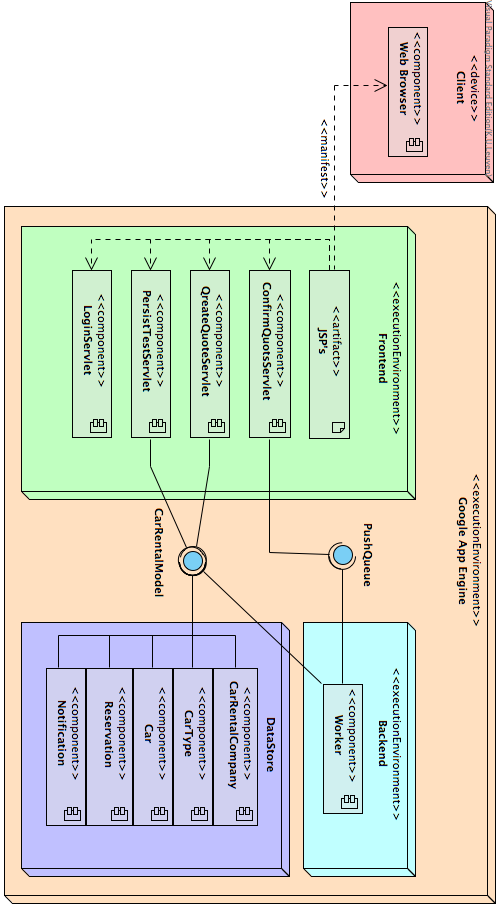
\includegraphics[width=\textwidth,height=\textheight,keepaspectratio]{Deployment_Diagram}
\end{figure}

\begin{figure}[h]
  \centering
    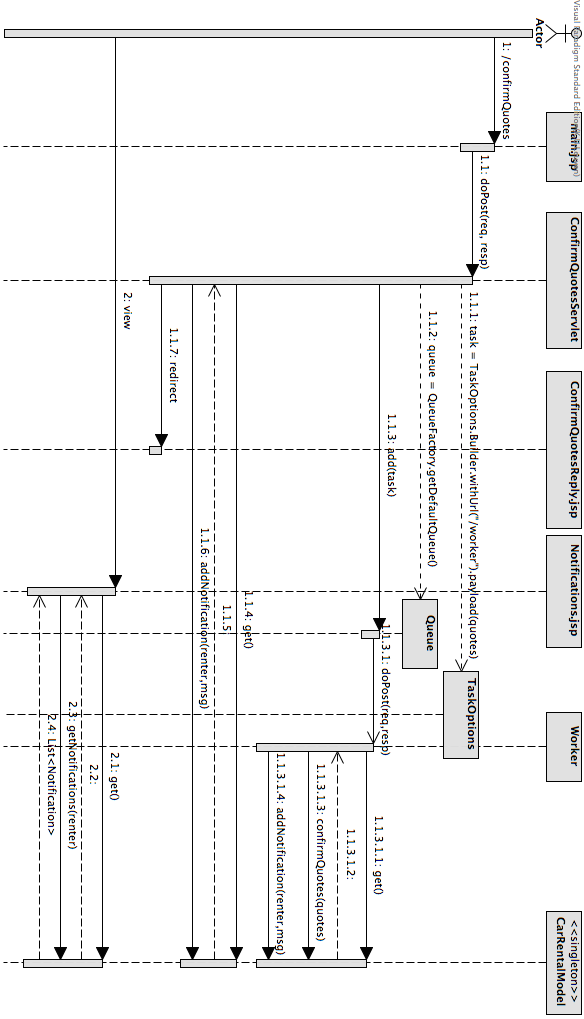
\includegraphics[width=\textwidth,height=\textheight,keepaspectratio]{Sequence_Diagram}
\end{figure}

% Emacs 24.3.1 (Org mode N/A)
\end{document}
